\section{Implementation}\label{sec:impl}


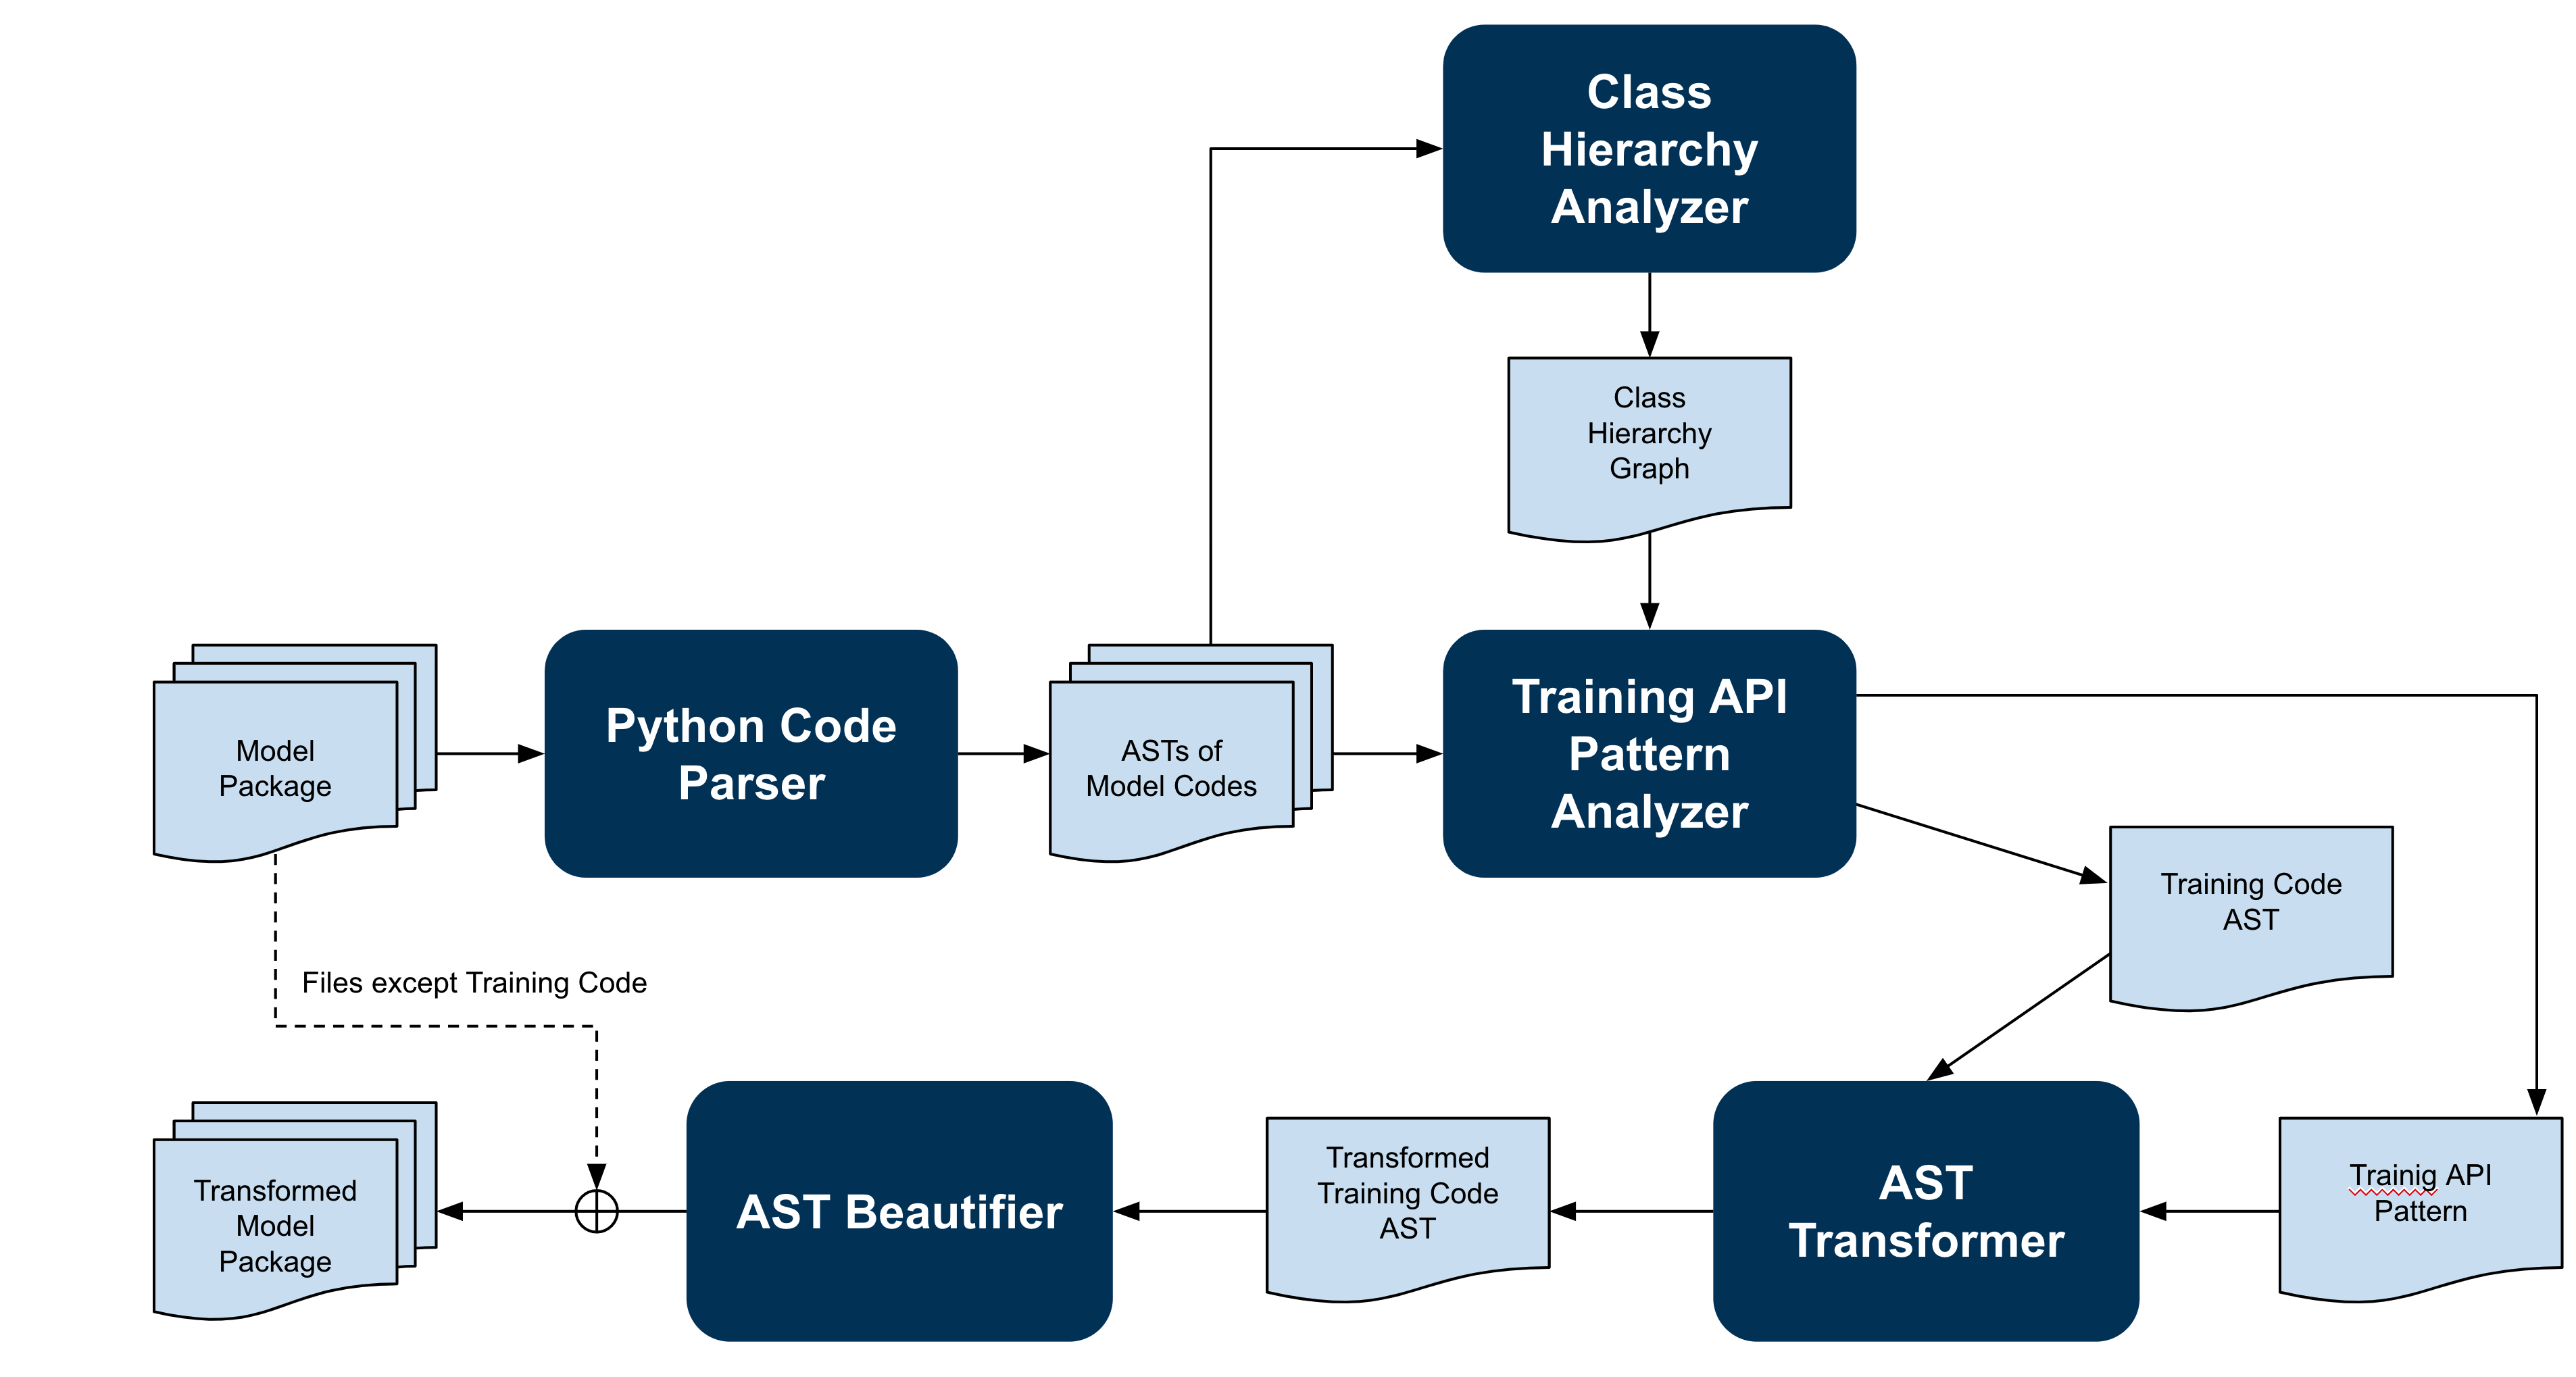
\includegraphics[width=15cm]{system_arch}

The figure illustrates the software architecture and workflow.
The software is composed of 5 modules:
Python code parser, class hierarchy analyzer,
training API pattern anlayzer, AST transformer, and AST beautifier.
The parser module parses Python codes in the input model package into 
a set of ASTs. Then the class hierarchy analyzer module 
produces a class hierarchy graph of the model package.
The training API pattern analyzer module receives the AST set and
the class hierarchy graph, identified the training code AST and
its training API pattern. The AST transformer module
transforms the training code AST according to the transformation rule.
The transformed training code AST is printed as a Python code in the
AST beautifier module, to be merged with the original model package
and become the transformed model package.

\subsection{Training API Pattern Analyzer}

The training API pattern analyzer module implements the training API
patterns and the training code categorization into the training API categories.
First, the code patterns of the traninig API patterns are implemented
in terms of pattern matching expressions.

-----------

(necessity of TAPA)

As mentioned in Section 2.1, user can choose which APIs to use
when building model using TensorFlow library.
However, different transformation rule should be applied
to different usage pattern of training API.
To apply appropriate rule to each model,
the training API pattern is analyzed before the transformation.

(categories of TAP)

First, we categorized the training API pattern into 4 categories:
Session/MonitoredSession, low-level API using TensorFlow1;
Estimator, high-level API using TensorFlow1;
DistributedGradientTape, low-level API using TensorFlow2;
and Keras, high-level API using TensorFlow2.
(TODO: show the category into a table)

(how TAPA work)

Each category has unique pattern of using training API.
For example, Keras pattern is 1) making instance of model and
2) call compile and fit method of that model.
Conversly, if call expressions of the method model.compile and model.fit are detected
where model is an instance of subclass of Model class in TensorFlow library,
we categorize it as Keras pattern.

(result of TAPA)

By using training API pattern analyzer, we can figure out the API pattern.
However, it is possible that model uses more than one categories of API pattern
such as using both low-level and high-level APIs.
In this case, we reject to transform because we assumes
that each model uses only one training API pattern in the transformation rule.

\subsection{AST Transformer}

The AST transformer module takes three input objects: a module AST,
a class hierarchy graph, and the training API usage summary.
The module AST represents the original training code, which will
be transformed into a distributed training code.
The class hierarchy graph represents the hierarchy between
user-defined classes and TensorFlow classes appear in the model code package.
The training API usage summary stores the training API category
information of the training code AST. Given these three inputs,
the AST transformer selects the appropriate transform function
for the training API category and apply it to the input AST.
In the transform function application, the pattern matching
and pattern guard utilizes the subclassing information
given by the CHG. 

